\documentclass{article}
\usepackage{tikz}
\usepackage{graphicx}
\graphicspath{{./images/}}
\usetikzlibrary{arrows.meta,shapes,automata,positioning}

\begin{document}

% \begin{tikzpicture}
% % Define the points of a regular pentagon
% \path (0,0) coordinate (origin);
% \path (0:1cm) coordinate (P0);
% \path (1*72:1cm) coordinate (P1);
% \path (2*72:1cm) coordinate (P2);
% \path (3*72:1cm) coordinate (P3);
% \path (4*72:1cm) coordinate (P4);
% % Draw the edges of the pentagon
% \draw (P0) -- (P1) -- (P2) -- (P3) -- (P4) -- cycle;
% % Add "spokes"
% \draw (origin) -- (P0) (origin) -- (P1) (origin) -- (P2)
% (origin) -- (P3) (origin) -- (P4);
% \end{tikzpicture}

% \begin{tikzpicture}
% \draw (0:1cm) -- (0:2cm)
% 	arc (0:60:2cm) -- (60:1cm)
% 	arc (60:0:1cm) -- cycle;
% \end{tikzpicture}

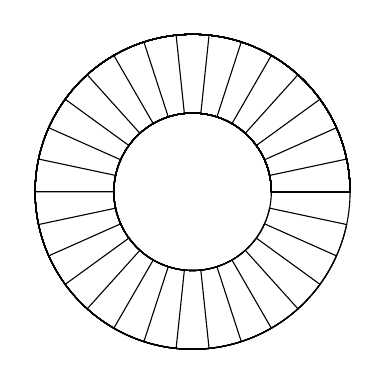
\begin{tikzpicture}
	\foreach \angle in {0,12,...,360}{
	% rm = angle
		% \path (5:\angle) coordinate (Q);
		\draw (0:1cm) -- (0:2cm)
			arc (0:\angle:2cm) -- (\angle:1cm)
			arc (\angle:0:1cm) -- cycle;
	}
\end{tikzpicture}

% 	\tikzstyle{every node}=[draw,shape=circle];
% 	\path (0:0cm) node (v0) {$v_0$};
% 	\path (0:1cm) node (v1) {$v_1$};
% 	\path (72:1cm) node (v2) {$v_2$};
% 	\path (2*72:1cm) node (v3) {$v_3$};
% 	\path (3*72:1cm) node (v4) {$v_4$};
% 	\path (4*72:1cm) node (v5) {$v_5$};
% 	\draw (v0) -- (v1)
% 	(v0) -- (v2)
% 	(v0) -- (v3)
% 	(v0) -- (v4)
% 	(v0) -- (v5);
% \end{tikzpicture}

 

% \frame{
% \begin{figure}
% \begin{center}
% 	\begin{tikzpicture}[shorten >=1pt,node distance=2cm,on grid,>={Stealth[round]},semithick,every state/.style={}]
% 	\node[state,initial]  (s_0)  					    {$s_0$};
% 	\node[state] at (3,0) (s_1) 					    {$s_1$};
% 	\node[state] at (6,0) (s_2) 					    {$s_2$};
	

% 	\path[->] (s_0) edge [loop above] node 			     {0,1}   (s_1)
% 			  (s_0) edge			  node	[above]		 {1}   	 (s_1)
% 			  (s_1) edge 			  node	[above]		 {0,1}   (s_2);
% 	\end{tikzpicture}
% 	\caption{
% 		X=\{$x$ $\in$ \{0,1\}$^{*}|$ the second symbol from the right is 1\}
% 	}

% \end{center}
% \end{figure}
% }

% \frame{
% \frametitle{Automaton $2$}
% \begin{figure}
% \begin{center}
% 	\begin{tikzpicture}[shorten >=1pt,node distance=2cm,on grid,>={Stealth[round]},semithick,every state/.style={}]
% 	\node[state,initial]   (s_0)  					    {$s_0$};
% 	\node[state] at (0,-2) (s_1) 					    {$s_1$};
% 	\node[state] at (2,0)  (s_2) 					    {$s_2$};
% 	\node[state] at (2,-2) (s_3) 					    {$s_3$};
	

% 	\path[->] (s_0) edge [loop above] node 			     {0}   (s_0)
% 			  (s_2) edge [loop above] node 			     {0}   (s_2)
% 			  (s_0) edge			  node	[above]		 {$\epsilon$}   	 (s_2)
% 			  (s_0) edge [bend left]	  node	[right]	 {1}   (s_1)
% 			  (s_1) edge [bend left]	  node	[left]	 {1}   (s_0)
% 			  (s_2) edge [bend left]	  node	[right]	 {1}   (s_3)
% 			  (s_3) edge [bend left]	  node	[left]	 {1}   (s_2);
% 	\end{tikzpicture}
% 	\caption{
% 		X=\{$x$ $\in$ \{0,1\}$^{*}|$ the second symbol from the right is 1\}
% 	}

% \end{center}
% \end{figure}
% }
 
\end{document} 
